\documentclass{scrreprt}

\usepackage{aligned-overset}
\usepackage{amsmath}
\usepackage{amsthm}
\usepackage{amssymb}
\usepackage{bm}
\usepackage[inline,shortlabels]{enumitem}
\usepackage{framed}
\usepackage{hyperref}
\usepackage[utf8]{inputenc}
\usepackage{multicol}
\usepackage{mathtools}
\usepackage{pdflscape}
\usepackage{physics}
\usepackage{polynom}
\usepackage{tabularx}
\usepackage[table]{xcolor}
\usepackage{titling}
\usepackage{fancyhdr}
\usepackage{xfrac}
\usepackage{pgfplots}

\pgfplotsset{compat = newest}
\usepgfplotslibrary{fillbetween}
\usetikzlibrary{calc}


\author{Karsten Lehmann}
\date{WiSe 2024/25}
\title{Übungsblatt 11\\INF-B-110, Lineare Algebra}

\setlength{\parindent}{0pt}

\setlength{\headheight}{26pt}
\pagestyle{fancy}
\fancyhf{}
\lhead{\thetitle}
\rhead{\theauthor}
\lfoot{\thedate}
\rfoot{Seite \thepage}

\begin{document}
\paragraph{Ü11.3 Eigenwerte und Eigenräume einer Spiegelung in $\mathbb{R}^2$}

Es sei $f \colon \mathbb{R}^2 \to \mathbb{R}^2$ die Spiegelung an der Geraden
$g = \text{Span}\qty\big{v}$ mit $v = \qty\big(2, 1) \in \mathbb{R}^2$.

\begin{enumerate}[(a)]
\item Veranschaulichen Sie sich diese Abbildung geometrisch und überlegen Sie
  damit, welche Eigenwerte $f$ hat und was die dazugehörigen Eigenräume sind.
  Geben Sie eine Basis $B' = \qty\big(u_1, u_2)$ von $\mathbb{R}^2$ aus
  Eigenvektoren von $f$ an.

  \subparagraph{Lsg.} Betrachtet werden die Vektoren
  \[
    u = \qty\big(1, 1)^T,
    v = \qty\big(2, 1)^T,
    w = \qty\big(-1, 2)^T,
  \]
  und deren Spiegelbilder $u'$, $v'$ und $w'$.

  \begin{tikzpicture}[scale=2]
    \begin{axis}[
      axis equal image,
      axis x line=center,
      axis y line=center,
      grid=both,
      xlabel={$\mathbb{R}$},
      xmin=-4.2,
      xmax=4.2,
      xtick distance=1,
      ylabel={$\mathbb{R}$},
      ymin=-4.2,
      ymax=4.2,
      ytick distance=1,
    ]
      \node[circle, draw, fill, minimum size=1mm, inner sep=0pt, label=above:{$u$}] (u) at (1, 1) {};
      \node[circle, draw, fill, minimum size=1mm, inner sep=0pt, label={5:$u'$}] (us) at ($({7/5}, {1/5})$) {};
      \node[circle, draw, fill, minimum size=1mm, inner sep=0pt, label=above:{$v, v'$}] at (2, 1) {};
      \node[circle, draw, fill, minimum size=1mm, inner sep=0pt, label=above:{$w$}] (w) at (-1, 2) {};
      \node[circle, draw, fill, minimum size=1mm, inner sep=0pt, label=below:{$w'$}] (ws) at (1, -2) {};
      \node at (3,2) {g};

      \draw (4.5,2.25) -- (-4.5,-2.25);
      \draw[dashed] (w) -- (ws);
      \draw[dashed] (u) -- (us);
    \end{axis}
  \end{tikzpicture}

  Somit hat $f$ die Eigenwerte $\lambda_1 = 1$ mit zum Beispiel dem Eigenvektor
  $v$ und $\lambda_2 = -1$ mit zum Beispiel dem Eigenvektor $w$.
  Nun sind $v$ und $w$ offensichtlich linear unabhängig und
  $B' = \qty\big(v, w)$ eine Basis von $\mathbb{R}^2$.

  \[
    \text{Eig}\qty\big(f, \lambda_1) = \text{Span}\qty\big{v}, \qquad
    \text{Eig}\qty\big(f, \lambda_2) = \text{Span}\qty\big{w}
  \]

\newpage
\item Bestimmen Sie die Darstellungsmatrix $A \coloneqq A_{BB}\qty\big(f)$ bzgl.
  der Standardbasis $B = \qty\big(e_1, e_2)$.

  \subparagraph{Lsg.} Die Standardbasis von $\mathbb{R}^2$ kann aus Eigenvektoren
  von $f$ dargestellt werden:
  \[
    \begin{pmatrix}
      1 \\
      0 \\
    \end{pmatrix} = \frac{2}{5} \cdot v - \frac{1}{5} \cdot w =
    \frac{2}{5} \cdot \begin{pmatrix}
      2 \\
      1 \\
    \end{pmatrix} - \frac{1}{5} \cdot \begin{pmatrix}
      -1 \\
      2 \\
    \end{pmatrix}
  \]
  und
  \[
    \begin{pmatrix}
      0 \\
      1 \\
    \end{pmatrix} = \frac{1}{5} \cdot v + \frac{2}{5} \cdot w =
    \frac{1}{5} \cdot \begin{pmatrix}
      2 \\
      1 \\
    \end{pmatrix} + \frac{2}{5} \cdot \begin{pmatrix}
      -1 \\
      2 \\
    \end{pmatrix}
  \]
  Nun ist
  \begin{flalign*}
    f\qty(\begin{pmatrix} 1 \\ 0 \end{pmatrix})
    &= f\qty(
      \frac{2}{5} \cdot \begin{pmatrix}
        2 \\
        1 \\
      \end{pmatrix} - \frac{1}{5} \cdot \begin{pmatrix}
        -1 \\
        2 \\
      \end{pmatrix}
    ) & \\
    \overset{f \text{ ist linear}}&= \frac{2}{5} \cdot f\qty(
      \begin{pmatrix}
        2 \\
        1 \\
      \end{pmatrix}
    ) - \frac{1}{5} \cdot f\qty(
      \begin{pmatrix}
        -1 \\
        2 \\
      \end{pmatrix}
    ) \\
    \overset{\text{Eigenvektoren}}&= \frac{2}{5} \cdot \lambda_1 \cdot \begin{pmatrix}
      2 \\
      1 \\
    \end{pmatrix} - \frac{1}{5} \cdot \lambda_2 \cdot \begin{pmatrix}
      -1 \\
      2 \\
    \end{pmatrix} \\
    &= \begin{pmatrix}
      \frac{4}{5} \\
      \frac{2}{5} \\
    \end{pmatrix} - \begin{pmatrix}
      \frac{1}{5} \\
      -\frac{2}{5}\\
    \end{pmatrix}
    = \begin{pmatrix}
      \frac{3}{5} \\
      \frac{4}{5} \\
    \end{pmatrix}
  \end{flalign*}
  und
  \begin{flalign*}
    f\qty(\begin{pmatrix} 0 \\ 1 \end{pmatrix})
    &= f\qty(
      \frac{1}{5} \cdot \begin{pmatrix}
        2 \\
        1 \\
      \end{pmatrix} + \frac{2}{5} \cdot \begin{pmatrix}
        -1 \\
        2 \\
      \end{pmatrix}
    ) & \\
    \overset{f \text{ ist linear}}&= \frac{1}{5} \cdot f\qty(
      \begin{pmatrix}
        2 \\
        1 \\
      \end{pmatrix}
    ) + \frac{2}{5} \cdot f\qty(
      \begin{pmatrix}
        -1 \\
        2 \\
      \end{pmatrix}
    ) \\
    \overset{\text{Eigenvektoren}}&= \frac{1}{5} \cdot \lambda_1 \cdot \begin{pmatrix}
      2 \\
      1 \\
    \end{pmatrix} + \frac{2}{5} \cdot \lambda_2 \cdot \begin{pmatrix}
      -1 \\
      2 \\
    \end{pmatrix} \\
    &= \begin{pmatrix}
      \frac{2}{5} \\
      \frac{1}{5} \\
    \end{pmatrix} + \begin{pmatrix}
      \frac{2}{5} \\
      -\frac{4}{5}\\
    \end{pmatrix}
    = \begin{pmatrix}
      \frac{4}{5} \\
      -\frac{3}{5} \\
    \end{pmatrix}
  \end{flalign*}
  Diese beiden Ergebnisse sind nun die Spalten der Darstellungsmatrix.
  \[
    A_{BB} = \begin{pmatrix}
      \frac{3}{5} & \frac{4}{5}  \\
      \frac{4}{5} & -\frac{3}{5} \\
    \end{pmatrix}
  \]

\item Bestimmen Sie die Darstellungsmatrix $D \coloneqq A_{B'B'}\qty\big(f)$
  bezüglich der Basis $B' = \qty\big(u_1, u_2)$.

  \subparagraph{Lsg.} Es ist $B' = \qty\big(v, w)$, das sind beides Eigenvektoren
  und somit enthält die Diagonale der Darstellungsmatrix deren Eigenwerte:
  \[
    D = \begin{pmatrix}
      \lambda_1 & 0         \\
      0         & \lambda_2 \\
    \end{pmatrix} = \begin{pmatrix}
      1 & 0  \\
      0 & -1 \\
    \end{pmatrix}
  \]

\newpage
\item Berechnen Sie eine invertierbare $2 \times 2$-Matrix $S$ über $\mathbb{R}$,
  so dass $D = S^{-1}AS$ gilt.
  Ist $S$ eindeutig bestimmt?

  \subparagraph{Lsg.} Nach der Vorlesung: Die Spalten von $S$ sind Eigenvektoren
  zu den Eigenwerten in $D$.
  \[
    S = \begin{pmatrix}
      2 & - 1 \\
      1 & 2   \\
    \end{pmatrix}, \qquad S^{-1} = \begin{pmatrix}
      \frac{2}{5}  & \frac{1}{5} \\
      -\frac{1}{5} & \frac{2}{5} \\
    \end{pmatrix}
  \]
  Und tatsächlich ist
  \[
    \begin{pmatrix}
      \frac{2}{5}  & \frac{1}{5} \\
      -\frac{1}{5} & \frac{2}{5} \\
    \end{pmatrix} \cdot \begin{pmatrix}
      \frac{3}{5} & \frac{4}{5}  \\
      \frac{4}{5} & -\frac{3}{5} \\
    \end{pmatrix} \cdot \begin{pmatrix}
      2 & -1 \\
      1 & 2  \\
    \end{pmatrix} = \begin{pmatrix}
      1 & 0  \\
      0 & -1 \\
    \end{pmatrix}
  \]
  Dabei ist $S$ nicht eindeutig bestimmt, die Matrix lässt sich ebenso aus
  anderen Eigenvektoren konstruieren.
  Zum Beispiel ist auch
  \[
    \begin{pmatrix}
      -\frac{2}{5} & -\frac{1}{5} \\
      \frac{1}{5}  & -\frac{2}{5} \\
    \end{pmatrix} \cdot \begin{pmatrix}
      \frac{3}{5} & \frac{4}{5}  \\
      \frac{4}{5} & -\frac{3}{5} \\
    \end{pmatrix} \cdot \begin{pmatrix}
      -2 & 1  \\
      -1 & -2 \\
    \end{pmatrix} = \begin{pmatrix}
      1 & 0  \\
      0 & -1 \\
    \end{pmatrix}
  \]

  \textbf{Alternativ nach der Übung:} $S$ ist die Matrix, die hilft von der
  Basis $B'$ zu $B$ zu wechseln.
  \[
    \qty(S^{-1}A_{BB}\qty\big(f)S)\qty\big(v)_{B'} = f\qty\big(v)_{B'}
  \]
  Somit $S = A_{B'B}\qty\big(id)$.
\end{enumerate}

\paragraph{Ü 11.4 Diagonalisierung von Matrizen}
\begin{enumerate}[(a)]
\item Berechnen Sie für die folgenden Matrizen $A$ alle Eigenwerte, finden Sie
  jeweils eine Basis aus Eigenvektoren von $A$ und eine invertierbare Matrix $S$,
  so dass $D \coloneq S^{-1}AS$ eine Diagonalmatrix ist.
  Geben Sie jeweils die Matrix $D$ an.
  \begin{enumerate}[(i)]
  \item $A \coloneqq \begin{pmatrix}
      -1 & 1 \\
      2  & 0 \\
    \end{pmatrix}$

    \subparagraph{Lsg.} Es ist
    \begin{flalign*}
      \det\qty\big(A - \lambda \cdot E_2) = \det\begin{pmatrix}
        -1 - \lambda & 1        \\
        2            & -\lambda \\
      \end{pmatrix}
      &= -\lambda\qty\big(-1 - \lambda) - 2 \\
      &= \lambda^2 + \lambda - 2 \\
      &= \qty\big(\lambda + 2)\qty\big(\lambda - 1)
    \end{flalign*}
    $\Rightarrow$ die Matrix hat die Eigenwerte $\lambda_1 = -2$ und
    $\lambda_2 = 1$.

    Nun ist
    \[
      \text{Ker}\qty\big(A - \lambda_1 \cdot E_2)
      = \text{Ker}\qty(\begin{pmatrix}
        1 & 1 \\
        2 & 2 \\
      \end{pmatrix})
      = \text{Span}\qty{\begin{pmatrix} 1 \\ -1 \end{pmatrix}}
    \]
    und
    \[
      \text{Ker}\qty\big(A - \lambda_2 \cdot E_2)
      = \text{Ker}\qty(\begin{pmatrix}
        -2 & 1 \\
        2 & -1 \\
      \end{pmatrix})
      = \text{Span}\qty{\begin{pmatrix} 1 \\ 2 \end{pmatrix}}
    \]
    Somit $S = \begin{pmatrix}
      1  & 1 \\
      -1 & 2 \\
    \end{pmatrix}$ und $D = \begin{pmatrix}
      -2 & 0 \\
      0  & 1 \\
    \end{pmatrix}$.

  \item $A = \begin{pmatrix}
      0 & 1  & 0 \\
      1 & 0  & 0 \\
      1 & -1 & 1 \\
    \end{pmatrix}$

    \subparagraph{Lsg.} Es ist
    \begin{flalign*}
      \det\qty\big(A - \lambda \cdot E_3) = \det\begin{pmatrix}
        -\lambda & 1        & 0           \\
        1        & -\lambda & 0           \\
        1        & -1       & 1 - \lambda \\
      \end{pmatrix}
      \overset{\text{Entwicklung nach 3. Spalte}}&=
      \qty\big(1 - \lambda)\det\begin{pmatrix}
        -\lambda & 1        \\
        1        & -\lambda \\
      \end{pmatrix} \\
      &= \qty\big(1 - \lambda)\qty\big(\lambda^2 - 1) \\
      &= \qty\big(1 - \lambda)\qty\big(\lambda + 1)\qty\big(\lambda - 1)
    \end{flalign*}
    $\Rightarrow$ die Matrix hat die Eigenwerte $\lambda_1 = -1$ und
    $\lambda_2 = 1$.

    Nun ist
    \[
      \text{Ker}\qty\big(A - \lambda_1 \cdot E_2)
      = \text{Ker}\qty(\begin{pmatrix}
        1 & 1  & 0 \\
        1 & 1  & 0 \\
        1 & -1 & 2 \\
      \end{pmatrix})
      = \text{Ker}\qty(\begin{pmatrix}
        1 & 1 & 0  \\
        0 & 0 & 0  \\
        0 & 1 & -1 \\
      \end{pmatrix})
      = \text{Span}\qty{\begin{pmatrix} -1 \\ 1 \\ 1 \end{pmatrix}}
    \]
    und
    \[
      \text{Ker}\qty\big(A - \lambda_2 \cdot E_2)
      = \text{Ker}\qty(\begin{pmatrix}
        -1 & 1   & 0 \\
        1  & -1  & 0 \\
        1  & -1  & 0 \\
      \end{pmatrix})
      = \text{Ker}\qty(\begin{pmatrix}
        1  & -1  & 0 \\
        0  & 0   & 0 \\
        0  & 0   & 0 \\
      \end{pmatrix})
      = \text{Span}\qty{
        \begin{pmatrix} 1 \\ 1 \\ 0 \end{pmatrix},
        \begin{pmatrix} 0 \\ 0 \\ 1 \end{pmatrix}
      }
    \]

    Somit $S = \begin{pmatrix}
      -1 & 1 & 0 \\
      1  & 1 & 0 \\
      1  & 0 & 1 \\
    \end{pmatrix}$ und $D = \begin{pmatrix}
      -1 & 0 & 0 \\
      0  & 1 & 0 \\
      0  & 0 & 1 \\
    \end{pmatrix}$.
  \end{enumerate}

\newpage
\item Von den folgenden Matrizen $M$ sind die angegebenen Eigenvektoren bekannt.
  Geben Sie jeweils alle Eigenwerte und die Dimension der zugehörigen Eigenräume
  an.
  Sind diese Matrizen diagonalisierbar?
  \begin{itemize}
  \item $M \coloneqq \begin{pmatrix}
      2 & 3 & 3 \\
      3 & 2 & 3 \\
      3 & 3 & 2 \\
    \end{pmatrix}$, $v_1 = \begin{pmatrix}
      2  \\
      -2 \\
      0  \\
    \end{pmatrix}$, $v_2 = \begin{pmatrix}
      3  \\
      0  \\
      -3 \\
    \end{pmatrix}$, $v_3 = \begin{pmatrix}
      -1 \\
      -1 \\
      -1 \\
    \end{pmatrix}$

    \subparagraph{Lsg.} Es ist
    \[
      M \cdot v_1 = \begin{pmatrix}
        2 & 3 & 3 \\
        3 & 2 & 3 \\
        3 & 3 & 2 \\
      \end{pmatrix} \cdot \begin{pmatrix}
        2  \\
        -2 \\
        0  \\
      \end{pmatrix} = \begin{pmatrix}
        -2  \\
        2 \\
        0  \\
      \end{pmatrix} = -1 \cdot v_1
    \]
    \[
      M \cdot v_2 = \begin{pmatrix}
        2 & 3 & 3 \\
        3 & 2 & 3 \\
        3 & 3 & 2 \\
      \end{pmatrix} \cdot \begin{pmatrix}
        3  \\
        0  \\
        -3 \\
      \end{pmatrix} = \begin{pmatrix}
        -3  \\
        0 \\
        3  \\
      \end{pmatrix} = -1 \cdot v_2
    \]
    \[
      M \cdot v_3 = \begin{pmatrix}
        2 & 3 & 3 \\
        3 & 2 & 3 \\
        3 & 3 & 2 \\
      \end{pmatrix} \cdot \begin{pmatrix}
        -1 \\
        -1 \\
        -1 \\
      \end{pmatrix} = \begin{pmatrix}
        -8  \\
        -8 \\
        -8  \\
      \end{pmatrix} = 8 \cdot v_3
    \]
    Somit besitzt $M$ die Eigenwerte $\lambda_1 = -1$ und $\lambda_2 = 8$ mit
    $\text{dim}\qty(\text{Eig}\qty\big(M, \lambda_1)) = 2$ und
    $\text{dim}\qty(\text{Eig}\qty\big(M, \lambda_2)) = 1$.

    Damit ist $M$ diagonalisierbar mit zum Beispiel $S = \begin{pmatrix}
      2  & 3  & -1 \\
      -2 & 0  & -1 \\
      0  & -3 & -1 \\
    \end{pmatrix}$ und $S^{-1}MS = \begin{pmatrix}
      -1 & 0  & 0 \\
      0  & -1 & 0 \\
      0  & 0  & 8 \\
    \end{pmatrix}$.

  \item $M \coloneqq \begin{pmatrix}
      0 & 0 & 0 & 0 \\
      0 & 1 & 0 & 0 \\
      0 & 0 & 1 & 1 \\
      0 & 0 & 0 & 1 \\
    \end{pmatrix}$, $v_1 = \begin{pmatrix}
      2 \\
      0 \\
      0 \\
      0 \\
    \end{pmatrix}$, $v_2 = \begin{pmatrix}
      0  \\
      -1 \\
      0  \\
      0  \\
    \end{pmatrix}$, $v_3 = \begin{pmatrix}
      0 \\
      0 \\
      2 \\
      0 \\
    \end{pmatrix}$, $v_4 = \begin{pmatrix}
      0 \\
      2 \\
      2 \\
      0 \\
    \end{pmatrix}$

    \subparagraph{Lsg.} Es ist
    \[
      M \cdot v_1 = \begin{pmatrix}
        0 & 0 & 0 & 0 \\
        0 & 1 & 0 & 0 \\
        0 & 0 & 1 & 1 \\
        0 & 0 & 0 & 1 \\
      \end{pmatrix} \cdot \begin{pmatrix}
        2 \\
        0 \\
        0 \\
        0 \\
      \end{pmatrix} = \begin{pmatrix}
        0 \\
        0 \\
        0 \\
        0 \\
      \end{pmatrix} = 0 \cdot v_1
    \]
    \[
      M \cdot v_2 = \begin{pmatrix}
        0 & 0 & 0 & 0 \\
        0 & 1 & 0 & 0 \\
        0 & 0 & 1 & 1 \\
        0 & 0 & 0 & 1 \\
      \end{pmatrix} \cdot \begin{pmatrix}
        0  \\
        -1 \\
        0  \\
        0  \\
      \end{pmatrix} = \begin{pmatrix}
        0  \\
        -1 \\
        0  \\
        0  \\
      \end{pmatrix} = 1 \cdot v_2
    \]
    \[
      M \cdot v_3 = \begin{pmatrix}
        0 & 0 & 0 & 0 \\
        0 & 1 & 0 & 0 \\
        0 & 0 & 1 & 1 \\
        0 & 0 & 0 & 1 \\
      \end{pmatrix} \cdot \begin{pmatrix}
        0 \\
        0 \\
        2 \\
        0 \\
      \end{pmatrix} = \begin{pmatrix}
        0 \\
        0 \\
        2 \\
        0 \\
      \end{pmatrix} = 1 \cdot v_3
    \]
    \[
      M \cdot v_4 = \begin{pmatrix}
        0 & 0 & 0 & 0 \\
        0 & 1 & 0 & 0 \\
        0 & 0 & 1 & 1 \\
        0 & 0 & 0 & 1 \\
      \end{pmatrix} \cdot \begin{pmatrix}
        0  \\
        2  \\
        2  \\
        0  \\
      \end{pmatrix} = \begin{pmatrix}
        0  \\
        2  \\
        2  \\
        0  \\
      \end{pmatrix} = 1 \cdot v_4
    \]
    Somit besitzt $M$ die Eigenwerte $\lambda_1 = 0$ und $\lambda_2 = 1$.
    Dabei sind $v_2, v_3$ und $v_4$ linear abhängig mit
    $-2 \cdot v_2 + v_3 = v_4$.

    Prüfen wird die Dimension der Eigenräume:
    \[
      \text{Ker}\qty\big(M - \lambda_1 \cdot E_4)
      = \text{Ker}\qty(\begin{pmatrix}
        0 & 0 & 0 & 0 \\
        0 & 1 & 0 & 0 \\
        0 & 0 & 1 & 1 \\
        0 & 0 & 0 & 1 \\
      \end{pmatrix})
      = \text{Ker}\qty(\begin{pmatrix}
        0 & 0 & 0 & 0 \\
        0 & 1 & 0 & 0 \\
        0 & 0 & 1 & 0 \\
        0 & 0 & 0 & 1 \\
      \end{pmatrix})
      = \text{Span}\qty{\begin{pmatrix} 1 \\ 0 \\ 0 \\ 0 \end{pmatrix}}
    \]
    und
    \[
      \text{Ker}\qty\big(M - \lambda_2 \cdot E_4)
      = \text{Ker}\qty(\begin{pmatrix}
        -1 & 0 & 0 & 0 \\
        0  & 0 & 0 & 0 \\
        0  & 0 & 0 & 1 \\
        0  & 0 & 0 & 0 \\
      \end{pmatrix})
      = \text{Span}\qty{
        \begin{pmatrix} 0 \\ 1 \\ 0 \\ 0 \end{pmatrix},
        \begin{pmatrix} 0 \\ 0 \\ 1 \\ 0 \end{pmatrix}
      }
    \]

    Somit findet sich keine Eigenvektorbasis bezüglich $M$ und die Matrix ist
    nicht diagonalisierbar.
  \end{itemize}
\end{enumerate}

\newpage
\paragraph{Ü 11.5 Ein diskretes dynamisches System}

Sogenannte ``Räuber-Beute-Systeme'' können vereinfach als \emph{diskretes
  dynamisches System} dargestellt werden.
Ein Beispiel dafür ist die gut untersuchte Beziehung zwischen Fleckenkauz und
Buschratte.
Seien $E_k$ und $R_k$ die Eulen- und die Rattenpopulation (in Tausend) zum
Zeitpunkt $k$, dann berechnen sich die Populationen zum Zeitpunkt $k + 1$ als:
\begin{flalign*}
  E_{k + 1} &= a \cdot E_k + b \cdot R_k \\
  R_{k + 1} &= c \cdot E_k + d \cdot R_k \\
\end{flalign*}
Berechnen Sie für die Startwerte
$s_1 = \qty\big(E_0, R_0)^T = \qty\big(10, 10)^T$,
$s_2 = \qty\big(30, 10)^T$ und $s_3 = \qty\big(10, 20)^T$ die Populationen
zum Zeitpunkt $k = 100$ für folgende Parameter:
\[
  \begin{pmatrix}
    a & b \\
    c & d \\
  \end{pmatrix} = \begin{pmatrix}
    0,3  & 0,6 \\
    -0,4 & 1,7 \\
  \end{pmatrix} \eqcolon A
  \text{ und }
  \begin{pmatrix}
    a & b \\
    c & d \\
  \end{pmatrix} = \begin{pmatrix}
    0,5  & 0,5 \\
    -0,5 & 1,5 \\
  \end{pmatrix} \eqcolon B
\]

\subparagraph{Lsg.} Es werden gesucht:
\begin{itemize}
\item $A^{100} \cdot s_1$, $A^{100} \cdot s_2$, $A^{100} \cdot s_3$
\item $B^{100} \cdot s_1$, $B^{100} \cdot s_2$, $B^{100} \cdot s_3$
\end{itemize}
Nun die Rechnung ...
\begin{itemize}
\item Für $A$
  \begin{flalign*}
    \det\qty\big(A - \lambda \cdot E_2) &= \det\begin{pmatrix}
      0,3 - \lambda & 0,6           \\
      -0,4          & 1,7 - \lambda \\
    \end{pmatrix} & \\
    &= \qty\big(0,3 - \lambda)\qty\big(1,7 - \lambda) + 0,24 \\
    &= \lambda^2 -2\lambda + 0,75 \\
    &= \qty\big(\lambda - 1,5)\qty\big(\lambda - 0,5)
  \end{flalign*}
  $\Rightarrow \lambda_1 = 1,5$ und $\lambda_2 = 0,5$.

  \newpage
  Nun ist
  \[
    \text{Eig}\qty\big(A, \lambda_1)
    = \text{Ker}\qty\big(A - \lambda_1 \cdot E_2)
    = \text{Ker}\qty\big(\begin{pmatrix}
      -1,2 & 0,6 \\
      -0,4 & 0,2 \\
    \end{pmatrix})
    = \text{Ker}\qty\big(\begin{pmatrix}
      1 & -\frac{1}{2} \\
      0 & 0            \\
    \end{pmatrix})
    = \text{Span}\qty{\begin{pmatrix} 1 \\ 2 \end{pmatrix}}
  \]
  und
  \[
    \text{Eig}\qty\big(A, \lambda_2)
    = \text{Ker}\qty\big(A - \lambda_2 \cdot E_2)
    = \text{Ker}\qty\big(\begin{pmatrix}
      -0,2 & 0,6 \\
      -0,4 & 1,2 \\
    \end{pmatrix})
    = \text{Ker}\qty\big(\begin{pmatrix}
      1 & -3 \\
      0 & 0  \\
    \end{pmatrix})
    = \text{Span}\qty{\begin{pmatrix} 3 \\ 1 \end{pmatrix}}
  \]

  Schließlich ist mit $S = \begin{pmatrix}
    1 & 3 \\
    2 & 1 \\
  \end{pmatrix}$ die Matrix $A$ diagonalisierbar:
  \[
    S^{-1}AS = \begin{pmatrix}
      1,5 & 0   \\
      0   & 0,5 \\
    \end{pmatrix} \coloneq D
  \]
  und
  \[
    A^{100} = SD^{100}S^{-1}
  \]
  Bevor man das ausrechnet sieht man lieber, dass $s_2$ und $s_3$ in den
  Eigenräumen von $A$ liegen.
  Somit ist $A^{100} \cdot s_2 = 0,5^{100} \cdot s_2 \approx \qty\big(0, 0)^T$
  und $A^{100} \cdot s_3 = 1,5^{100} \cdot s_3$.

  Schließlich ist noch $s_1 = \frac{1}{5}s_2 + \frac{2}{5}s_3$ und somit
  \[
    A^{100} \cdot s_1 = \frac{0,5^{100}s_2 + 2 \cdot 1,5^{100}s_3}{5}
    \overset{0,5^{100} \longrightarrow 0}\approx \frac{1,5^{100}}{5} \cdot 2 \cdot s_3
  \]

  \textbf{Alternativ nach der Übung:} Rechne $SD^{100}S^{-1}$ weiter:
  \begin{flalign*}
    \begin{pmatrix}
      1 & 3 \\
      2 & 1 \\
    \end{pmatrix} \cdot \begin{pmatrix}
      1,5^{100} & 0         \\
      0        & 0,5^{100} \\
    \end{pmatrix} \cdot \frac{1}{5} \begin{pmatrix}
      -1 & 3  \\
      2  & -1 \\
    \end{pmatrix}
    &= \begin{pmatrix}
      1,5^{100}         & 3 \cdot 0,5^{100} \\
      2 \cdot 1,5^{100} & 0,5^{100}         \\
    \end{pmatrix} \cdot \frac{1}{5} \begin{pmatrix}
      -1 & 3  \\
      2  & -1 \\
    \end{pmatrix} \\
    &= \frac{1}{5} \begin{pmatrix}
      1,5^{100}         & 3 \cdot 0,5^{100} \\
      2 \cdot 1,5^{100} & 0,5^{100}         \\
    \end{pmatrix} \cdot \begin{pmatrix}
      -1 & 3  \\
      2  & -1 \\
    \end{pmatrix} \\
    &= \frac{1}{5} \begin{pmatrix}
      6 \cdot 0,5^{100} - 1,5^{100}          & 3 \cdot 1,5^{100} - 3 \cdot 0,5^{100} \\
      -2 \cdot 1,5^{100} + 2 \cdot 0,5^{100} & 6 \cdot 1,5^{100} - 6 \cdot 0,5^{100} \\
    \end{pmatrix} \\
    \overset{0,5^{100} \longrightarrow 0}&\approx \frac{1}{5} \begin{pmatrix}
      - 1,5^{100}         & 3 \cdot 1,5^{100}  \\
      - 2 \cdot 1,5^{100} & 6 \cdot 1,5^{100} \\
    \end{pmatrix} \\
    &\approx A^{100}
  \end{flalign*}
  Nun ist
  \[
    A^{100} \cdot s_1 =
    \frac{1}{5} \begin{pmatrix}
      - 1,5^{100}        & 3 \cdot 1,5^{100} \\
      -2 \cdot 1,5^{100} & 6 \cdot 1,5^{100} \\
    \end{pmatrix} \cdot \begin{pmatrix}
      10 \\
      10 \\
    \end{pmatrix} = \frac{1,5^{100}}{5} \begin{pmatrix}
      20 \\
      40 \\
    \end{pmatrix}
  \]
  \[
    A^{100} \cdot s_2 =
    \frac{1}{5} \begin{pmatrix}
      - 1,5^{100}        & 3 \cdot 1,5^{100} \\
      -2 \cdot 1,5^{100} & 6 \cdot 1,5^{100} \\
    \end{pmatrix} \cdot \begin{pmatrix}
      30 \\
      10 \\
    \end{pmatrix} = \frac{1,5^{100}}{5} \begin{pmatrix}
      0 \\
      0 \\
    \end{pmatrix}
  \]
  \[
    A^{100} \cdot s_3 =
    \frac{1}{5} \begin{pmatrix}
      - 1,5^{100}        & 3 \cdot 1,5^{100} \\
      -2 \cdot 1,5^{100} & 6 \cdot 1,5^{100} \\
    \end{pmatrix} \cdot \begin{pmatrix}
      10 \\
      20 \\
    \end{pmatrix} = \frac{1,5^{100}}{5} \begin{pmatrix}
      50  \\
      100 \\
    \end{pmatrix}
  \]
  An den Ergebnissen sieht man nun, dass in etwa doppelt so viele Ratten wie
  Eulen benötigt werden.

  Weiter nähern sich solche Systeme häufig/immer dem Eigenraum mit dem größten
  Eigenwert an.

\item Für $B$
  \begin{flalign*}
    \det\qty\big(A - \lambda \cdot E_2) &= \det\begin{pmatrix}
      0,5 - \lambda & 0,5           \\
      -0,5          & 1,5 - \lambda \\
    \end{pmatrix} & \\
    &= \qty\big(0,5 - \lambda)\qty\big(1,5 - \lambda) + 0,25 \\
    &= \lambda^2 -2\lambda + 1 \\
    &= \qty\big(\lambda - 1)\qty\big(\lambda - 1)
  \end{flalign*}
  $\Rightarrow \lambda_1 = 1$.

  Nun ist
  \[
    \text{Eig}\qty\big(B, \lambda_1)
    = \text{Ker}\qty\big(B - \lambda_1 \cdot E_2)
    = \text{Ker}\qty\big(\begin{pmatrix}
      -0,5 & 0,5 \\
      -0,5 & 0,5 \\
    \end{pmatrix})
    = \text{Ker}\qty\big(\begin{pmatrix}
      1 & -1 \\
      0 & 0  \\
    \end{pmatrix})
    = \text{Span}\qty{\begin{pmatrix} 1 \\ 1 \end{pmatrix}}
  \]
  Leider findet sich so keine Basis aus Eigenvektoren.

  Immerhing liegt $s_1$ im Eigenraum von $B$ und somit lässt sich
  $B^{100} \cdot s_1 = 1^{100} \cdot s_1= s_1$ schnell ermitteln.
\end{itemize}
\end{document}
